%!TEX root = ../BoYu-Dissertation.tex
\graphicspath{{Figures/}}

\chapter{Knowledge Representation and Updating} % (fold)
\label{cha:knowledge_reprsentation_and_updating}
In this chapter, we provide details about the first component of our computational framework for event-driven awareness promotion, i.e. how the computer constructs and develops the knowledge representation of collaborative activities within the event-driven processes. We first provide a computational representation of collaborative activities using the PlanGraph model. Then, we discuss the specification and typology of events in our approach. Based on these two knowledge components, we discuss the the knowledge updating process, in which they are mutually developed. On one hand, the knowledge representation of an collaborative activity is updated by reacting to the various external and internal events, so that it always reflects the current state of the collaborative activity. On the other hand, during the updating process, the system's knowledge about the events are also enriched by interpreting their meanings in the context of the collaborative activity.

\section{Representing collaborative activities} % (fold)
\label{sec:representing_the_field_of_work}
In this section, we present the knowledge representation of collaborative activities based on PlanGraph model. By modeling an collaborative activity within a PlanGraph, the various entities and relations as we formalized in Section \ref{sub:structure_of_a_collaborative_activity} can be represented as different components of the PlanGraph. Then we show how the local scopes and dependency networks can be derived from the PlanGraph model, making use of the knowledge about these entities and relations.

\subsection{The PlanGraph model} % (fold)
\label{sub:the_plangraph_model}
The PlanGraph model with its basis in the SharedPlans theory is designed to represent the dynamic knowledge in the human-computer collaboration \cite{Cai2005}. In general, a PlanGraph represents the knowledge about a collaborative activity towards a shared goal in a hierarchical way (Figure \ref{fig:plangraph}). The root of a PlanGraph is the overall goal of the actors in a collaborative activity, which is decomposed recursively into actions through the adoption of recipes. The PlanGraph as a whole represents the shared plan corresponding to the top-level collaborative activity, while each sub-tree with an action as the root represents the shared plan for that action. A PlanGraph is composed of three types of nodes: (1) \emph{action} nodes represent all the actions and sub-actions in the collaborative activity; (2) \emph{parameter} nodes represent informational or physical objects that are used by actions; (3) \emph{condition} nodes represent states of affairs in the world that the actors would like to achieve.

There are several ways that these three types of nodes can be connected in a PlanGraph:
\begin{enumerate}
	\item An action can be decomposed into several parameters, conditions, and sub-actions, where the parameters indicate all the informational or physical objects that will be used by the action. All these parameters need to satisfy their own constraints before the action can be performed, and they are accessible by all the subsidiary actions at the same level. The conditions under an action correspond to all the constraints that need to be satisfied before the action or any sub-actions can be performed.  
	\item Each parameter can be decomposed into sub-actions and conditions. The sub-actions of a parameter are used to assign values for the parameter, i.e. they are used to satisfy the knowledge-precondition on the parameter. The conditions attached to a parameter are other preconditions that need to be satisfied before the parameter is ready to be used by upper action.
	\item Each condition can only be decomposed into subsidiary actions that are used to ensure the condition is satisfied.
\end{enumerate}

The PlanGraph model also encodes the actors that are participated in each action. Because the relations between actors and actions can be many-to-many, i.e. an actor can work on multiple actions, and one action can involve multiple actors, we represent knowledge of actors within their relations towards each action. Each action node in a PlanGraph includes several attributes to store the relations with participating actors as defined in Section \ref{ssub:relations}: \emph{Intentions} records the different intention relations of each actor towards the action. \emph{Capabilities} indicates the level of capability of each actor to perform the action.

\begin{figure}[htbp] %  figure placement: here, top, bottom, or page
   \centering
   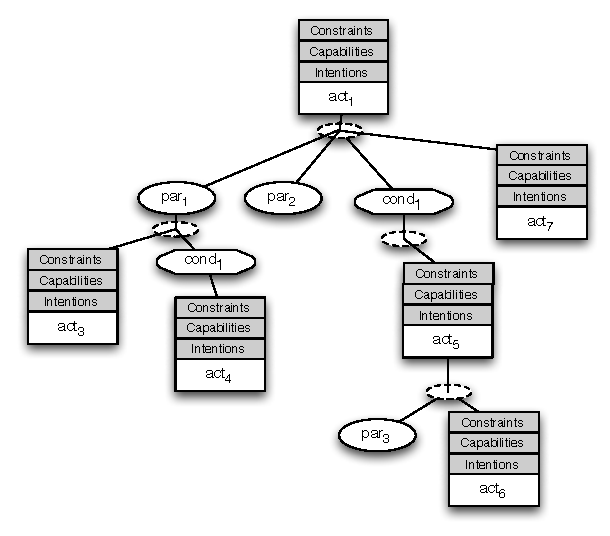
\includegraphics{plangraph.pdf} 
   \caption{Structure of a PlanGraph}
   \label{fig:plangraph}
\end{figure}

The PlanGraph model has been used to model the human-computer collaboration as a collaborative activity in several applications, e.g. the natural conversational interface to geospatial databases \cite{Cai2005}, collaborative dialog-based system to communicate vague spatial concepts \cite{Cai2003}, and context-aware mobile mapping \cite{yu2010using}. However, in order to model the collaborative activities among human actors, several modifications to the original PlanGraph model have been made in this study:

\begin{enumerate}
 	\item First, the parameter nodes in the original PlanGraph model are mainly used to represent knowledge preconditions, i.e. they represent the knowledge needed for the action to be performed. In this study, we extend the concept of parameter to represent both the physical and informational resources that are needed for the action.
 	\item We extend the original PlanGraph model to explicitly represent conditions as standalone nodes. This allows us to model the indirect dependency relations among actions between human actors. For instance, even though $act_1$ does not indicate a higher level goal of $act_2$, it can still depends on the $act_2$ because $act_2$ satisfies a condition that is required for performing $act_1$.
 	\item The original PlanGraph model for human-computer collaboration treats the computer system as an actor with its own intentions and beliefs. However, as we focus on tracking the states and relations among human actors' actions, we do not explicitly model the computer's beliefs and intentions.
 \end{enumerate} 
% subsection the_plangraph_model (end)

\subsection{Representing elements and relations} % (fold)
\label{sub:representing_activities}
The PlanGraph model allows us to represent the basic entities and relations in a collaborative activity. The actions, actors, and resources are first-class objects in the PlanGraph model, and the multiple relations among then can be represented as structural relations in the PlanGraph model (Table \ref{tab:basic_rel_pg}). 

\paragraph*{Actors} % (fold)
\label{par:actors_in_plangraph}
Each actor is represented as an object with a unique \emph{ID} in the PlanGraph model. Each actor object in the PlanGraph maintain the current state of the corresponding actor, such as the name, the location, the role of the actor, and the expertise he/she has. Each actor object also maintains a list of actions that the actor is currently participated in.
% paragraph actors_in_plangraph (end)

\paragraph*{Actions} % (fold)
\label{par:actions_in_plangraph}
Actions are directly modeled as a type of nodes in the hierarchical structure of the PlanGraph. Each action node has several important attributes:
\begin{enumerate}
	\item The \emph{goal} of the action is represented as an expression, indicating the expected effect of the action when it is successfully performed.
	\item The \emph{execution state} of the action records the current state of the action towards its performance, e.g. whether it has been started, successfully performed, or in the progress.
	\item The \emph{recipe} points to the current recipe to perform the action if the current recipe is selected from the knowledge base. Each recipe specifies a particular way to perform the action. In the case the recipe is identified by human actors on the fly, this could be empty.
	\item The \emph{Intentions} and \emph{Capabilities} record the different relations between participating actor towards the action.
	\item The \emph{Constraints} record the relations between sub-actions, such as temporal orders between them, or whether they can be optional.
\end{enumerate}
% paragraph actions_in_plangraph (end)

\paragraph*{Resources} % (fold)
\label{par:resources_in_plangraph}
Resources are assigned to parameter nodes as values. Parameter nodes can be collective or individual. A collective parameter includes a collection of resources with the same type as its value, for instance, a parameter representing all the victims in the same rescue operation. All the resources assigned to the same parameter node need to satisfy conditions that are linked to the resource node.
% paragraph resources_in_plangraph (end)

\paragraph*{Relations between actors and their actions} % (fold)
\label{par:relations_between_actors_and_their_actions}
The relations between actors and their actions can be directly retrieved from the \emph{Intentions} and \emph{Capabilities} attributes attached to each action, recording the different relations between participating actors towards the action.
% paragraph relations_between_actors_and_their_actions (end)

\paragraph*{Relations between actions} % (fold)
\label{par:relations_between_actions}
The two major types of relations between actions are composition and precedence. The former is directly encoded in the hierarchical structure of a PlanGraph. Each action node has an list of its sub-actions under current plan. The precedence relation that reflects the temporal order of performing two actions is encoded in the \emph{constraints} attribute of their parent action node.
% paragraph relations_between_actions (end)

\paragraph*{Relations between resources and actions} % (fold)
\label{par:relations_between_resources_and_actions}
The relations between resources and actions can be inferred from the structural relations between action nodes and parameter nodes in a PlanGraph. The resources assigned to a parameter node underlying an action node can be consumed by the action and all its sub-actions. The actions that are used to assign values to a parameter or achieve preconditions of the parameter can manipulate all the resources attached to the parameter node.
% paragraph relations_between_resources_and_actions (end)

{\footnotesize
\begin{longtable}{>{\raggedright}p{1.5in}>{\raggedright}p{4in}}
\toprule 
Relation & Structure in PlanGraph\tabularnewline
\midrule 
$Pot.Int(ar,act)$ \par $Int.Th(ar,act)$ \par $Int.to(ar,act)$ \par $Perform(ar,act)$ & search the \emph{Intentions} slot attached to each action node: 
\par 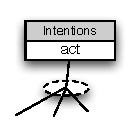
\includegraphics{intentions.pdf}\tabularnewline
\midrule 
$Knows(ar,act)$ \par $Able(ar,act)$ \par $Workable(ar,act)$ & search the \emph{Capability} slot attached to each action node: 
\par 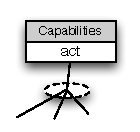
\includegraphics{capabilities.pdf}\tabularnewline
\midrule 
$Sub.Act(act_1, act_2)$ &  $act_1$ is a subsidiary action node under $act_2$: 
\par 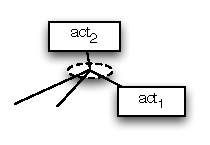
\includegraphics{sub_act.pdf} \tabularnewline
\midrule 
$Precedes(act_1, act_2)$ &  $act_1$ and $act_2$ as ordered siblings: 
\par 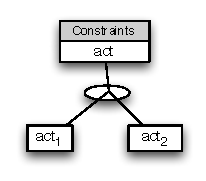
\includegraphics{precedes.pdf}\tabularnewline
\midrule 
$Consume(act, res)$ & a parameter node representing a resource $res$ and  a action node $act$ as siblings: 
\par 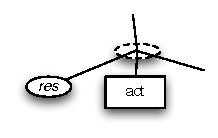
\includegraphics{consumes.pdf}\tabularnewline
\midrule 
$Produces(act, res)$ &  $act$ is a subsidiary action node under the parameter node representing a resource $res$: 
\par 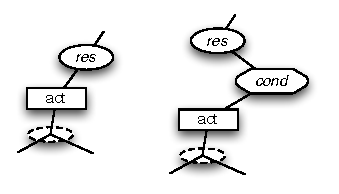
\includegraphics{produces.pdf}\tabularnewline
\bottomrule
\caption{Representing basic relations in PlanGraph}
\label{tab:basic_rel_pg}
\end{longtable}
}
% subsubsection representing_relations (end)
% subsection representing_activities (end)

\subsection{Constructing local scopes} % (fold)
\label{sub:representing_local_scopes}
Based on the definition of local scopes in Section \ref{sub:local_scope_of_work}, the local scope of an actor can be dynamically constructed by depth-first traversal through the PlanGraph structure to search for all the actions that are related to the actor through intention or capability relations.

We define a procedure $BUILD\textrm{-}LS$ that takes an actor object $ar$ and a PlanGraph $PG$ to construct both the local scope of intentions $LSI$ and local scope of capabilities $LSC$ for the actor. We define a sub-procedure $ADD\textrm{-}To\textrm{-}LS$ that takes an actor object $ar$ and an action node $act$ in the PlanGraph to add the action to the local scope $LSI$ or $LSC$ based on whether the corresponding intention or capability relation exists. The $ADD\textrm{-}TO\textrm{-}LS$ procedure then calls itself recursively on all the children nodes to traverse to the deeper levels in the PlanGraph. In this way, the process to construct the local scopes $BUILD\textrm{-}LS$ starts with the initialization of $LSI$ and $LSC$, and then recursively calls $ADD\textrm{-}TO\textrm{-}LS$ from the root node of the PlanGraph.

{\footnotesize
\begin{algorithm}
\begin{algorithmic}[1]
\Procedure{BUILD-LS}{$ar,PG$}
	\State $LSI\gets [\:], LSC\gets [\:]$
	\State $root\gets PG.root$
	\State $ADD\textrm{-}TO\textrm{-}LS(ar, root)$\Comment{start the recursion from $root$}
\EndProcedure
\Procedure{ADD-TO-LS}{$ar,act$}
	\ForAll{$int$ \textbf{in} $act.intentions$}\Comment{check the current node}
   		\If{$int.actor == ar$}
   			\State $LSI.add(ar, act, int)$
   		\EndIf
	\EndFor
	\ForAll{$cap$ \textbf{in} $act.capabilities$}
   		\If{$cap.actor == ar$}
   			\State $LSC.add(ar, act, cap)$
   		\EndIf
	\EndFor
	\ForAll{$par$ \textbf{in} $act.parameters$}\Comment{recursion on parameters}
   		\ForAll{$subact$ \textbf{in} $par.subacts$}
   			\State $ADD\textrm{-}TO\textrm{-}LS(ar, subact)$
		\EndFor
	\EndFor
	\ForAll{$cond$ \textbf{in} $act.conditions$}\Comment{recursion on conditions}
   		\ForAll{$subact$ \textbf{in} $cond.subacts$}
   			\State $ADD\textrm{-}TO\textrm{-}LS(ar, subact)$
		\EndFor
	\EndFor
	\ForAll{$subact$ \textbf{in} $act.subacts$}\Comment{recursion on subacts}
   		\State $ADD\textrm{-}TO\textrm{-}LS(ar, subact)$
	\EndFor
\EndProcedure
\end{algorithmic}
\end{algorithm}
}
% subsection representing_local_scopes (end)

\subsection{Constructing dependency network} % (fold)
\label{sub:representing_dependencies}
From the PlanGraph model, we can also dynamically construct the corresponding dependency network to represent how the actions are dependent on each other. Formally, a dependency network $DN=(V(DN), E(DN))$ is defined as a directed graph with the following characteristics:
\begin{enumerate}
	\item $V(DN)=\{ACT \cup PARAM \cup COND\}$ is the set of all the nodes in the dependency network, all the \emph{dependers} and \emph{dependees} are action nodes $ACT$, and the \emph{dependums} can be any parameter $RES$ or condition nodes $COND$. 
	\item The set $E(DN)$ is a set of links between the nodes. Each link can be represented as a pair of nodes in $V(DN)$, i.e. $E(DN) \to V(DN) \times V(DN)$. The link can indicate a direct dependency between two action nodes, or a incoming link that connects a \emph{depender} and \emph{dependum}, or an outgoing link that connects a \emph{dependum} and \emph{dependee}.
\end{enumerate}

The construction of dependency network can also be achieved by depth-first traversal through the PlanGraph model to search for all the action-action and action-resource relations. We define a procedure $BUILD\textrm{-}DN$ that constructs a dependency network from a PlanGraph $PG$. As the set of nodes $V(DN)$ can be calculated from the set of links $E(DN)$ by removing all the duplicates, the $BUILD\textrm{-}DN$ procedure focuses on building $E(DN)$. We define a sub-procedure $ADD\textrm{-}To\textrm{-}DN$ that takes an action node $act$ in the PlanGraph to add dependencies that starting from $act$, i.e. to find all the dependencies in which the $act$ is the \emph{depender}.

{\footnotesize
\begin{algorithm}
\begin{algorithmic}[1]
\Procedure{BUILD-DN}{$PG$}
	\State $E\gets [\:]$
	\State $root\gets PG.root$
	\State $ADD\textrm{-}TO\textrm{-}DN(root)$\Comment{start the recursion from $root$}
\EndProcedure
\Procedure{ADD-TO-DN}{$act$}
	\ForAll{$subact$ \textbf{in} $act.subacts$}\Comment{check for Sub.Act}
   		\State $E.add(act, subact)$
	\EndFor

	\If{$act.hasParent()$}
		\ForAll{$constr$ \textbf{in} $act.parent.constraints$}\Comment{check for Precedes}
			\If{$constr.next == act$}
   				\State $E.add(act, constr.prev)$ 
   			\EndIf
		\EndFor
		\ForAll{$par$ \textbf{in} $act.parent.parameters$}\Comment{check for parameters}
   			\ForAll{$subact$ \textbf{in} $par.subacts$}
   				\State $E.add(act, par), E.add(par, subact)$
			\EndFor
		\EndFor
		\ForAll{$cond$ \textbf{in} $act.parent.conditions$}\Comment{check for conditions}
   			\ForAll{$subact$ \textbf{in} $cond.subacts$}
   				\State $E.add(act, cond), E.add(cond, subact)$
			\EndFor
		\EndFor
   	\EndIf

	\ForAll{$par$ \textbf{in} $act.parameters$}\Comment{recursion on parameters}
   		\ForAll{$subact$ \textbf{in} $par.subacts$}
   			\State $ADD\textrm{-}TO\textrm{-}DN(subact)$
		\EndFor
	\EndFor
	\ForAll{$cond$ \textbf{in} $act.conditions$}\Comment{recursion on conditions}
   		\ForAll{$subact$ \textbf{in} $cond.subacts$}
   			\State $ADD\textrm{-}TO\textrm{-}DN(subact)$
		\EndFor
	\EndFor
	\ForAll{$subact$ \textbf{in} $act.subacts$}\Comment{recursion on subacts}
   		\State $ADD\textrm{-}TO\textrm{-}DN(subact)$
	\EndFor
\EndProcedure
\end{algorithmic}
\end{algorithm}
}
% subsection dependency_relations_in_the_activity_structure (end)
% section representing_the_field_of_work (end)

\section{Representing events} % (fold)
\label{sec:representing_events}
In Section \ref{ssub:the_concept_of_events}, we define \emph{`events'} to refer to the computerized entities that are used in an awareness system to represent knowledge about either real world \emph{`occurrence'} or the results of \emph{`awareness'} processes. In this section, we focus on how events are computationally represented in this study. Although they share the same representational structure in general, different types of events are represented differently. In the following, we first describe the general representational structure of events, then discuss the major event types, and their differences in representation.

\subsection{Structure of events} % (fold)
\label{sub:defining_events}
We follow many existing event processing systems to represent each event as a structured object consisting of a named set of attributes \cite{Mhl2010}. Formally, an event $e$ is a nonempty set of \emph{attributes} $\{a_1, a_2, ..., a_n\}$, where each $a_i$ a name/value pair $(n_i, v_i)$ with name $n_i$ and value $v_i$. It is assumed that names are unique, i.e., $i\ne j \Rightarrow n_i\ne n_j$, and that there exists a function that uniquely maps each $n_i$ to a data type $T_i$ that is the type of the corresponding value $v_i$.

The set of attributes for each event should help answer questions such as: What occurrence or awareness aspect it refers to? When did it happen? Where did it happen? What other information is associated with its happening? The answers to these questions are usually depend on the type of event they are associated with. An \emph{event type} is a generalization for a set of event objects that have the same semantic intent and same structure \cite{Etzion2010}, i.e. they share the same set of attributes, but may have different values. Each \emph{event type} has a unique event type identifier. In this study we use simple descriptive text strings for these identifiers, for example the phrase \emph{``LocationChanged''} identifies an event type that can describe any instance of an object's location change. Identifying the set of \emph{event types} is an application specific task, as actors in different applications have different awareness needs and capabilities to detect events. We describe the major event types that are supported in this study in Section \ref{sub:event_types}.

While arbitrary attributes can be included in each event type, we can group them into three categories, following the definitions in \cite{Etzion2010} (Figure \ref{fig:event_structure}):

\begin{enumerate}
	\item The \emph{header} consists of generic information about the event, such as the event type, occurrence time, etc. The header attributes are not specific to a particular event type, rather shared by all event types.
	\item The \emph{payload} contains a collection of attributes carrying the data that describes the actual occurrence. Unlike header attributes independent of the actual event type, the payload attributes are defined per event type. 
	\item An event can also contain free-format \emph{open content} information that provides a mechanism that the awareness system can use to enrich an event object with extra contextual information, such as human-readable explanation, multi-media content etc.
\end{enumerate}

\begin{figure}[htbp] %  figure placement: here, top, bottom, or page
   \centering
   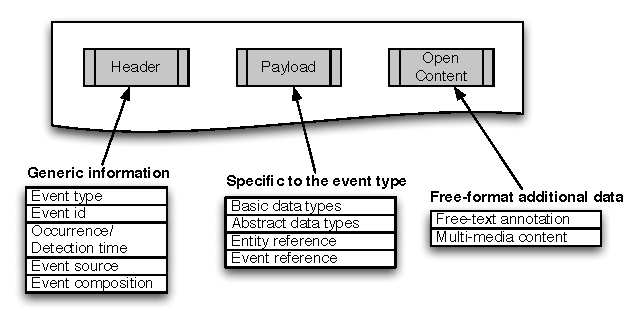
\includegraphics{event_structure.pdf} 
   \caption{The structure of an event (adapted from \cite{Etzion2010} p.63)}
   \label{fig:event_structure}
\end{figure}

\paragraph*{Header} % (fold)
\label{par:header}
The header of an event contains the common attributes that are included in every event object. Unlike payload or open content that are optional, a header is required for every event representation. In general, the header of an event needs to include the following attributes:

\begin{enumerate}
	\item \emph{Event type}. This attributes stores the event type identifier that uniquely identifies the event type of this event.
	\item \emph{Event identifier}. This is a unique identifier for each individual event object.
	\item \emph{Occurrence/detection time}. The occurrence time is the time when the real world occurrence happens. In some cases, the event producer might not be able to determine the time when the event actually occurred. For example, if the producer examines the state of some external entity only at periodic intervals. In such cases, the detection time is used instead, recording the time at which the event became known by the event producer. 
	\item \emph{Event source}. This is the entity that originates this event. This can be either an external sensor, or a human actor in the collaborative system.
	\item \emph{Event composition}. This is a boolean attribute that denotes whether the specific event is a composite event or not. A composite event is one whose payload is made up of several other event instances.
\end{enumerate}
% paragraph header (end)

\paragraph*{Payload} % (fold)
\label{par:payload}
The attributes that make up the event payload are used to carry the data that describes the actual occurrence. The set of attributes included in each event is a variable that depends on the corresponding event type. There are several types of data that can be included as payload attributes:
\begin{enumerate}
	\item \emph{Basic data types}. The value in an payload attribute can simply be in the basic data types, such as string, numeric boolean, date/time etc.
	\item \emph{Abstract data types}. Attributes can also have abstract data types that are structures composed of other data types. For example, many events includes a geographic attribute to records the whereabout of the represented real world occurrence. This attribute can be a point-based representation as a latitude/longitude pair, or more complicated as a route or a geographic area.
	\item \emph{Entity reference}. Instead of records the information directly in an attribute, the event can also records information by pointing to entities represented in the collaborative activities. For example, an \emph{`ActionPerformed'} event may use the reference to the action node stored in the PlanGraph model to indicate which action has been performed.
	\item \emph{Event reference}. Some events may contain references to other events. For example, a composite event may use the event references to record the primitive events that it is composed of.
\end{enumerate}
% paragraph payload (end)

\paragraph*{Open content} % (fold)
\label{par:open_content}
The open content of an event can include any attributes an awareness system can use to provide additional contextual information about the event. For example, it is used in the awareness externalization process to allow the actors to provide human-readable explanation of their interpretations.
% paragraph open_content (end)

% subsection defining_events (end)
\subsection{Event types} % (fold)
\label{sub:event_types}
As we argue in Section \ref{ssub:the_concept_of_events} that \emph{events} can be used to represent both description of real world \emph{occurrences} and externalization of human actors' internal \emph{awareness} knowledge, a fundamental distinction should be made between these two categories of events, we call the former \emph{external events}, and the latter {internal events}. The distinction between external events and internal events are important, because (1) they require different representational structures, i.e. the payloads of events have different sets of attributes; (2) they are consumed differently by the system when updating the knowledge representation; (3) and they are treated differently in  human users' awareness processes as well. 

Another distinction to make is the difference between \emph{primitive events} and \emph{composite events}. Composite events prevent the users from being overwhelmed by a large number of primitive event by providing them a higher-level abstraction \cite{Mhl2010}. Generally, a composite event is made up of several other events (either primitive or composite), according to a specification of relations between them. 

In the following, we first describe the major primitive event types, both external and internal, and then discuss the composite events as a special event type with its own payload structure.

\subsubsection{External events} % (fold)
\label{ssub:external_events}
As we conceptualize a collaborative environment as consisting of a variety of entities and relations, external events can be defined to indicate any kinds of changes on either these entities or relations. 

\paragraph*{Events on entities} % (fold)
\label{par:events_on_entities_}
We define each external event on an individual entity as a semantic function that changes the entity's property or state. We follow the general event ontology proposed in \cite{Kaneiwa2007} to define the following categories of external events on individual entities:

\begin{enumerate}
	\item \emph{State Change}. An event is a state change event if the occurrence yields a change of state on an entity. All the possible states of an entity are usually can be expressed as a discrete state machine, and each state transition indicates a possible state change event. For example, Figure \ref{fig:action_exec_state_trans} shows the transition diagram with all the possible execution states of an action. Each valid transition in the diagram can be considered as a state change event.
	\begin{figure}[htbp] %  figure placement: here, top, bottom, or page
   	\centering
   	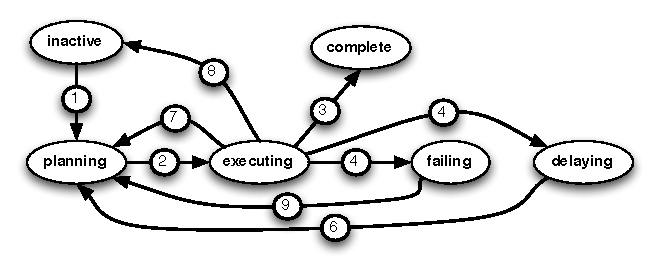
\includegraphics{action_exec_state_trans.pdf} 
   	\caption{Execution state transition of an action}
   	\label{fig:action_exec_state_trans}
	\end{figure}
	\item \emph{Existential Change over Time}. An event indicates an existential change over time if its occurrence changes the existence of an entity in temporal order, e.g. an entity did not exist in the past but it exists now.
	\item \emph{Existential Change over Space}. An event indicates an existential change over space if its occurrence changes the existence of an entity depending on its movement through space, e.g. an entity existed at location A, but now exists at location B. 
	\item \emph{Value Comparison}. Another common class of external events are comparison events to indicate changes on attribute values of an entity. They can used to indicate whether an attribute value is equal, unequal, greater than, or less than a fixed threshold, or the same attribute value in the past. 
\end{enumerate}
% paragraph events_on_entities_ (end)

\paragraph*{Events on relations} % (fold)
\label{par:events_on_relations}
Events on relations are used to indicate whether some relations between entities hold. For example, an event with the type \emph{`ResourceAssigned'} indicates an assignment relation between a resource and an action becomes holding, i.e. the resource is now assigned for performing the action. Therefore, the types of external events on relations depend on the possible types of relations that can be identified in the domain. 

Generally, the basic relations between entities in the real world can be divided into three categories: spatial, temporal, and conceptual \cite{Tomaszewski2010}.

\begin{enumerate}
	\item The spatial relations link the entities through their spatial positions. The basic types of spatial relations have been well studied in the literature of geographic information systems, include binary topological \cite{egenhofer1994deriving}, directional \cite{frank1991qualitative}, and distance relations \cite{hernandez1995qualitative}. Topological relations is a particular subset of geometric relations that are preserved under topological transformations such as translation, rotation, and scaling. Some examples are relations indicating whether one entity disjoints, meets, overlaps, or contains another entity. Directional relations indicate the relative direction between two entities, such as one is at north of the other. Distance relations link entities based on their proximity in the space, such as one is within a certain range of another. 
	\item The temporal relations link the entities based on their temporal positions. The basic types of temporal relations are considered in the literature on temporal reasoning \cite{allen1994actions}, including binary topological, ordering, and distance relations \cite{Andrienko2011}.
	\item The conceptual relations are an umbrella term that covers all the different types of organizational, structural, or social relations between entities in a particular collaborative activity. 
\end{enumerate}

From the basic types of relations, more complex types of relations can be built, such as
density (clustering, dispersion), arrangement (e.g. sequence in time or alignment in space) and spatial-temporal relations. The latter are composed of spatial and temporal relations and represent changes of spatial relations over time: approaching or going away, entering or exiting, following, keeping distance, concentrating or dissipating and so on.
% paragraph events_on_relations (end)

Figure \ref{fig:external_events} shows an upper level typology of the external events that can be defined on entities and relations in a collaborative environment.
\begin{figure}[htbp] %  figure placement: here, top, bottom, or page
	\centering
	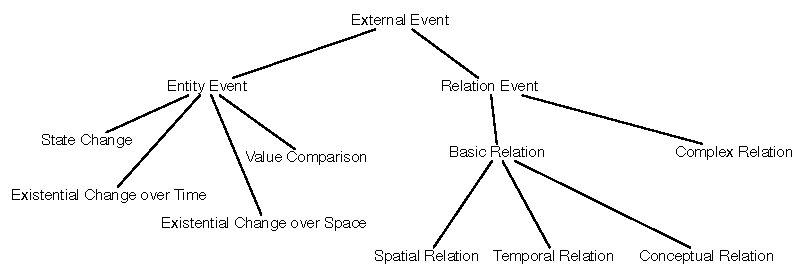
\includegraphics{external_events.pdf} 
	\caption{An upper level typology of external events}
	\label{fig:external_events}
\end{figure}

\paragraph*{Relevance to the collaborative activities} % (fold)
\label{par:relevance_to_the_field_of_work}
 Although the number of external events that could be possibly identified is infinite, not all of them are relevant to the human actors' working context. As a result, the goal of identifying external events in an awareness system focuses on finding a subset of event types that could possibly contribute to the understanding of supported collaborative activities. In general, we believe that the relevance of external events to a collaborative activity can be analyzed based on the different functional roles they can play in updating the knowledge about the collaborative activity. If the occurrence of an external event can imply some change in the collaborative activity, it should be treated as relevant. Based on our conceptualization of collaborative activities, we can identify the following function roles for external events:

 \begin{enumerate}
 	\item \emph{Direct change to entities in a collaborative activity}. External events can indicate changes on individual entities that are modeled in a collaborative activity, i.e. the property or state change of the resources, actors, or actions. For example, a state change event can be used to indicate the change of execution state for an action. Location change events can be used to describe an actor's movement. 
 	\item \emph{Direct change to relations in a collaborative activity}. Some external events are directly related to the various relations between resource, actors, and actions as we described in Section \ref{ssub:relations}. For example, an external event type indicating the constitution relation between two entities can be used to describe the $Sub.Act$ relation between two actions, i.e. one action is a subsidiary action to perform another one. The assignment relation event type can be used to describe relations between an action and a resource, i.e. the resource has been assigned to the performance of the action. 
 	\item \emph{Goal activation}. Aside from the two cases that external events can be directly linked to the entities and relations in a collaborative activity, external events can also impact the collaborative activity by activate the goals to perform actions. For example, an external event indicating that the fire alarm is ringing will activate the human actor's goal to escape from the office. In this case, the fire alarm is not directly linked to any entities in the human actor's activities, rather it motivates the actor to perform a new action.
 	\item \emph{Implied changes to entities and relations}. In some cases, external events can also provide some evidence implying changes in the entities and relations in a collaborative activity. For example, instead of a state change event directly showing the action to delivery a resource to an actor has been completed, it could be implicitly inferred from a spatial relation event that indicates the resource is now located at the actor's location. Similarly, an external event indicating the occurrence of a traffic blocking between the resource's current location and the actor's implies the delivery action is in trouble.
 \end{enumerate}
% paragraph relevance_to_the_field_of_work (end)
% subsubsection external_events (end)
\subsubsection{Internal events} % (fold)
\label{ssub:internal_events}
Internal events are used to describe the results of human actors' awareness processes. Unlike external events that can describe changes in any entities and relations in a collaborative activity, internal events describe the changes of human actors' internal mental states towards the collaborative activity. Internal events are usually derived from external events to indicate human actors' interpretations on them. In this study, we identify two types of internal events: \emph{intention} events and \emph{belief} events. 

An \emph{intention} event indicates a human actor's adoption of certain intention towards some action in a collaborative activity. Figure \ref{fig:intention_event} shows the basic structure of an intention event. The payload of an intention event include three required attributes: an intention type indicating whether it's $Pot.Int$, $Int.Th$, or $Int.To$, a reference to the actor who adopts this intention, and a reference to the intended action. An optional free-text attribute is included in the open content part, where the human actor can provide the rationale for adopting the corresponding intention.
\begin{figure}[htbp] %  figure placement: here, top, bottom, or page
	\centering
	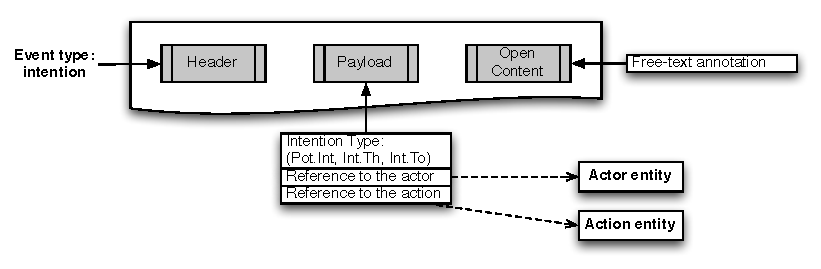
\includegraphics{intention_event.pdf} 
	\caption{Structure of an intention event}
	\label{fig:intention_event}
\end{figure}

A \emph{belief} event describes a human actor's belief in some entities or relations in a collaborative activity. For example, it can be used to indicate an actor's belief that an action has been successfully performed, or the belief that the actor has the capability to perform an action. As belief events usually refer to some changes on entities or relations in a collaborative activity, we represent each belief event by embedding an external event representing the content of the belief in its payload (Figure \ref{fig:belief_event}). However, unlike the standalone external event that indicates a change that has already happened, the change described in a belief event can be something that will happen in the future. These belief events can be used to represent the results of the human actor's projection process, i.e. what the actor expects to happen in the future. There are two attributes in a belief event's open content part: the free-text explanation of this belief, and a confidence level to describe how confident the actor is about this belief.
\begin{figure}[htbp] %  figure placement: here, top, bottom, or page
	\centering
	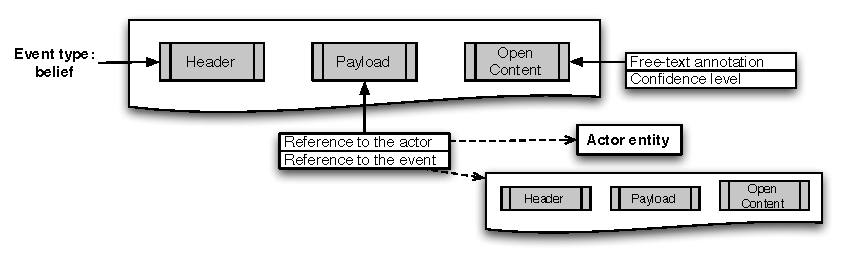
\includegraphics{belief_event.pdf} 
	\caption{Structure of a belief event}
	\label{fig:belief_event}
\end{figure}
% subsubsection internal_events (end)

\subsubsection{Composite events} % (fold)
\label{ssub:composite_events}
Composite events are a special type of events that can consist of several other events. The subsidiary events can be external or internal. Besides the list of subsidiary events, a composite event needs to also describe how these sub-events are combined together. In a simple case, a composite event can occur only when all the sub-events occur. Moreover, a composite event can occur when some of the sub-events occur, but some do not. Or it occurs when any of the sub-events occurs. A more complicated composite event language can be found in \cite{Mhl2010} that includes different relations between sub-events, such as negation, concatenation, sequence, iteration etc. To describe the composition pattern, a specific payload attribute needs to be included in a composite event's representation (Figure \ref{fig:composite_event}).
\begin{figure}[htbp] %  figure placement: here, top, bottom, or page
	\centering
	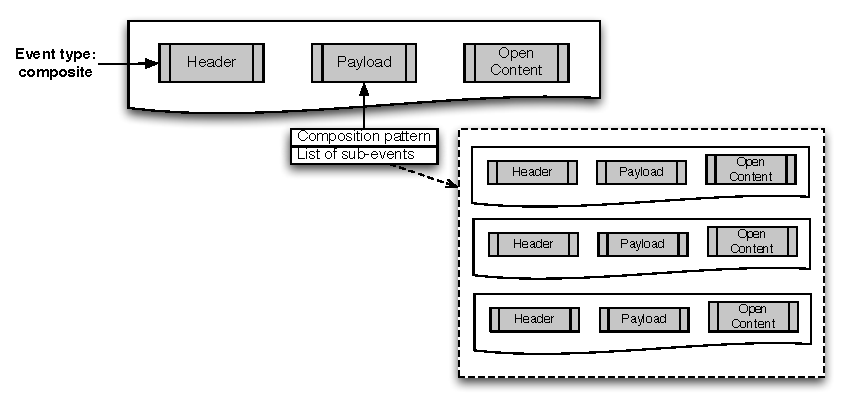
\includegraphics{composite_event.pdf} 
	\caption{Structure of a composite event}
	\label{fig:composite_event}
\end{figure}
% subsubsection composite_events (end)
% subsection event_types (end)
% section representing_events (end)

\section{The knowledge updating process} % (fold)
\label{sec:knowledge_updating_process}
The knowledge updating process describes how the aforementioned knowledge representations of collaborative activities and events are mutually developed. Each time when a new event is input into the system, it triggers the knowledge updating process. The knowledge updating process performs two important tasks: (1) it decides on how the input event influences the current collaborative activity and updates the correspondent in the PlanGraph model; (2) it augments the event representation by establishing the links between the event and the corresponding entities in the PlanGraph, and records the development of the event based on the system's reasoning.

\paragraph*{Updating knowledge about the collaborative activity} % (fold)
\label{par:updating_the_plangraph}
In general, the knowledge updating is a four-step process: \emph{association}, \emph{assessment}, \emph{elaboration}, and \emph{propagation}, through which the knowledge representation of the collaborative activity, i.e. the PlanGraph model is updated (Figure \ref{fig:updating_plangraph}).
\begin{figure}[htbp] %  figure placement: here, top, bottom, or page
	\centering
	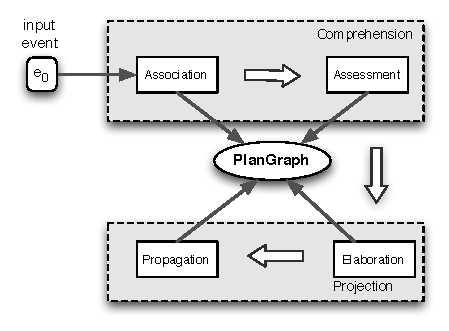
\includegraphics{updating_plangraph.pdf} 
	\caption{The knowledge updating process}
	\label{fig:updating_plangraph}
\end{figure}

\begin{enumerate}
	\item \emph{Association}. The knowledge updating starts with the association of an event with the PlanGraph model. In this step, the system searches the PlanGraph for an appropriate match between the input event and the entities and relations in the collaborative activity. If a match is found, the system uses the information stored in the event to update the corresponding entities or relations in the PlanGraph.
	\item \emph{Assessment}. The second step is to assess how the event can lead to new changes in the collaborative activity. For instance, it may trigger new actions that need to be performed, or change the current states of existing actions. 
	\item \emph{Elaboration}. Based on the assessment of the event, the elaboration step is to reason about the system's expectation on how the newly added action should be decomposed into sub-actions, or what actors will be potentially involved in these new actions. This is usually performed with domain specific knowledge, such as recipes of action performance, and role specifications of actors.
	\item \emph{Propagation}. The propagation step focuses on evaluating how the current change can be possibly propagated to other actions in the collaborative activity because of the dependencies among actions. 
\end{enumerate}

The four steps of knowledge updating process share some commonality with the human actor's awareness development processes. The \emph{association} and \emph{assessment} steps are similar to the \emph{comprehension} process, where human actors comprehend or understand the relevance of awareness information in relation to their tasks and goals. The \emph{elaboration} and \emph{propagation} can be considered as the projection of states in the near future. In this way, we can think of the knowledge updating process as the computer system's awareness development process. The only difference is that, as the human actors usually only have partial knowledge about the collaborative activity, the computer system aims to possess the knowledge of the whole collaborative activity through knowledge updating.

One thing to note is that not every event will be processed in all the four steps. Some external event may not directly link to any entities in the collaborative activity, or the system does not have the complete knowledge to assess its implications in the collaborative activity. In such case, the event may be passed directly to human actors for interpretation. The result of human actors' interpretation may generates a new internal event that starts a new round of knowledge updating, in which the system's knowledge is updated.
% paragraph updating_the_plangraph (end)

\paragraph*{Updating knowledge about the event} % (fold)
\label{par:updating_the_event_representation}
As we emphasize in the beginning, while the knowledge about the collaborative activity is updated by the new event, the event itself is also developed during the system's reasoning process. For example, in the \emph{assessment} step, an external event \emph{`TrafficBlocked'} causes the system to believe that the action to deliver a resource cannot be achieved. One one hand, this causes the system to modify the state of the delivery action in the PlanGraph. Meanwhile, the system generates a new internal event describing the system's belief about the state change of the delivery action. Later, in the \emph{propagation} step, the system may generate another internal event to indicate that because of the state change of the delivery action, the action that depends on the resource delivery will also be impacted. In this way, the original event is derived into a chain of events as the knowledge updating proceeds.

To record the development of an event in the knowledge updating process, we define an \emph{event chain} $EC$ as an ordered sequence of events: $EC=(e_0, e_1, e_2, ...)$. In the beginning of the knowledge updating process, there may be only one event $e_0$, i.e the original external event in the event chain $EC$. As the knowledge updating proceeds, more events are added to the chain. In the assessment step, the system may generate \emph{derived events} indicating the system's beliefs on how the other entities or relations in the collaborative activity have been changed due to the original event. In the propagation step, the system predicates the future state changes, and attaches more \emph{anticipatory events} to the event chain. Figure \ref{fig:knowledge_updating} shows how an event is developed into an event chain in the knowledge updating process.

\begin{figure}[htbp] %  figure placement: here, top, bottom, or page
	\centering
	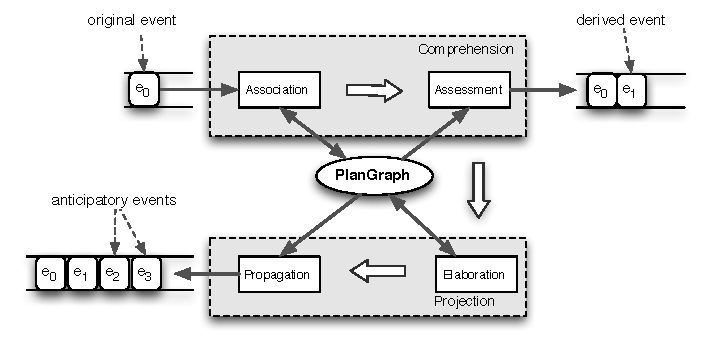
\includegraphics{knowledge_updating.pdf} 
	\caption{The development of an event chain}
	\label{fig:knowledge_updating}
\end{figure}

In order to record an \emph{event chain}, we add three additional attributes in the \emph{open content} section of every event in the chain:

\begin{enumerate}
 	\item A text string (\emph{label}) indicates the functional role of the event in the event chain, i.e. whether the event is an \emph{original} event, a \emph{derived} event, or an \emph{anticipatory} event.
 	\item An event reference (\emph{prevEvent}) points to its preceding event in the event chain. It can be optional when the current event is the \emph{original} event, but required for \emph{derived} and \emph{anticipatory} events.
 	\item An event reference (\emph{nextEvent}) points to its succeeding event in the event chain. It can be optional if the current event is at the end of the event chain.
 \end{enumerate} 

 Figure \ref{fig:event_chain_structure} shows how the additional information about the event chain is included in an event's representation. 

\begin{figure}[htbp] %  figure placement: here, top, bottom, or page
	\centering
	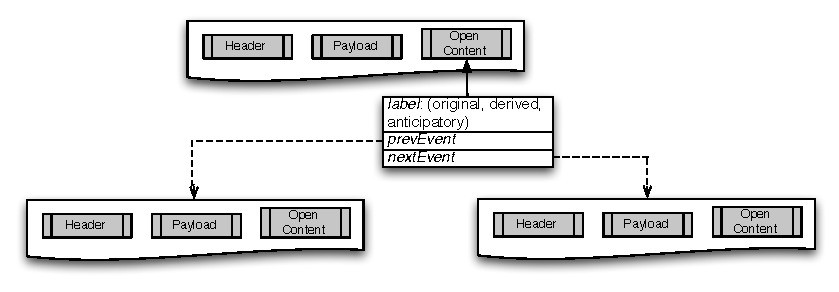
\includegraphics{event_chain_structure.pdf} 
	\caption{Event structure in an event chain}
	\label{fig:event_chain_structure}
\end{figure}
% paragraph updating_the_event_representation (end)

\subsection{Association} % (fold)
\label{sub:association}
The knowledge updating starts with establishing associations between the input event and entities and relations in the current PlanGraph model representing the collaborative activity, and uses the information carried by the event to update the PlanGraph model. Based on the different event types, the association is conducted differently.

If the event is an \emph{external event} on entities, we consider the following two cases:
\begin{enumerate}
	\item If the event indicates an existential change over time, the event is directly passed through to the assessment step, as the entity related to this event did not exist in the past.
	\item Otherwise, we search all the PlanGraph nodes to find any match with the entity described in the event based on their unique identifiers. If a match is found, we update the attribute information attached with the PlanGraph node based on the event type. If it is a state change event, we change the state of th node. If it is an existential change over space, we update the location information of the node. If it is a value comparison event, we update the corresponding attribute value. After updating the node, we add an entity reference in the event object, so that the event is direct linked to the matched PlanGraph node.
\end{enumerate}

If the event is an \emph{external event} on relations, we check for the following cases:
\begin{enumerate}
	\item If the event indicates a resource assignment relation, i.e. a resource $res_1$ is assigned to the performance of an action $act_1$. we search all the action nodes in the PlanGraph to find any match with $act_1$. If a match is found, we search for the parameters of $act_1$ in the PlanGraph to find any of them has the same resource type as $res_1$ and then assign the values of $res_1$ to the parameter. After that, we add an entity reference pointing to the parameter node in the event's payload. 
	\item If the event is related to a structural relation, e.g. an action $act_2$ is a sub-action of another action $act_1$. we search all the action nodes in the PlanGraph to find any match with $act_1$. If a match is found, we create a new node with the information described in $act_2$, and then add an entity reference pointing to this new node into the event's payload. This can be applied to other decomposition relations, such as a sub-action to achieve a condition, or a new parameter added to an existing action.
\end{enumerate}

If the event is an \emph{internal event}, we consider the following cases:
\begin{enumerate}
	\item If the event is an \emph{intention event}, we search all the action nodes in the PlanGraph to find any match with the action entity described in the event. If a match is found, we search for the \emph{Intentions} attribute associated with the action node to find whether any existing actor has the same identifier as the actor described in the event. If so, we update the intention type based on the intention event. Otherwise, we add the actor and the corresponding intention into the \emph{Intentions} associated with the action node. After that, we add an entity reference pointing to the action node in the event's payload. 
	\item If the event is a \emph{belief event} about an actor's capability to perform an action, we search all the action nodes in the PlanGraph to find any match with the action entity described in the event. If a match is found, we search for the \emph{Capabilities} associated with the action node to find whether any existing actor has the same identifier as the actor entity described in the event. If so, we update the capability type based on the belief event. Otherwise, we add the actor and the corresponding capability level into the \emph{Capabilities} associated with the action node. After that, we add an entity reference pointing to the action node in the event's payload. 
	\item If the event is other \emph{belief events}, we apply the association rules directly on the subsidiary event describing the content of the belief. 
\end{enumerate}

In sum, if an association between the event and the PlanGraph model is found, two tasks are performed. First, the corresponding PlanGraph entity or relation is updated based on the new information carried by the event. Second, the event is enriched by directly linking to the corresponding PlanGraph node, as the result of which the context of origin for this event is identified. However, not all the events can be directly associated with the PlanGraph model. Some external events may describe changes on the entities that are not currently in the PlanGraph, but implicitly impact the collaborative activity by motivating new actions or implying changes. These events will be passed to the assessment step for further analysis. 
% subsection association (end)

\subsection{Assessment} % (fold)
\label{sub:assessment}
In the assessment step, each event is evaluated to check how it can lead to new changes in the collaborative activity implicitly, where inference becomes necessary. For example, an external event indicating that a resource is now located at an actor's position implicitly indicates the successful performance of the resource delivery action to the actor. In this case, a new event showing the state change of the resource delivery action will be derived and added to the event chain along with the original event.

The knowledge stored in the PlanGraph allows the system to perform some routine assessment tasks that are universal in different application domains:
\begin{enumerate}
	\item \emph{Goal conditions on action nodes}. If an event describes changes on entities or relations that are included in an action's goal condition, the system can evaluate the action's goal condition. If the goal condition becomes holding because of this event, the system derives a new state change event on this action, and adds it into the event chain.
	\item \emph{Condition nodes}. If an event describes changes on entities or relations that are included in a condition node, the system can evaluate the condition node. If the condition becomes holding or no longer holding because of this event, it derives a new state change event on this condition, and pushes it into the event chain. 
	\item \emph{Parameter nodes}. If an event describes changes on a resource that is assigned to a parameter node, the system can evaluate the parameter's subsidiary conditions. If a  condition becomes holding or no longer holding because of this event, it derives a new state change event on this parameter, and adds it into the event chain.
\end{enumerate}

The second type of tasks that the system can perform during the assessment process is to check whether the event can activate new actions that need to be added to the collaborative activity. This type of events is usually called \emph{triggering events}, as they are often not directly associated with any existing nodes in the PlanGraph, but will trigger some new action to be added. For example, every time a new victim is found in an emergency response operation will trigger a new rescue action to be performed. In this case, the initial event about the discovery of a new victim cannot be associated with any existing actions, but asks for a new action to be performed. The assessment of action activation requires a set of pre-defined domain-specific activation rules, so that every event is searched through the activation rules to find whether it satisfies any of the conditions. If so, a new action is added to the PlanGraph, and a new derived event is generated to indicate the activation of the new action.

Furthermore, the assessment step can involve more sophisticated inference techniques, such as spatio-temporal reasoning \cite{Bennett}, pattern recognition \cite{zelnik2001event}, or case-based reasoning \cite{jakobson2004towards}, to enhance the system's reasoning capabilities. However, these reasoning techniques often require a large amount of domain knowledge to be modeled, and lack flexibility to handle unexpected events. As a result, in the assessment step, we design the system to focus on more reliable low-level routine inferences, and leave the complex, higher level assessment tasks to the human actors. Hence, some events may not be considered as contributing to the collaborative activity by the system in the assessment process. Rather, they are sent to human actors for interpretation. The result of human interpretation generates new events that are then sent back to the system to update the system's knowledge.
% subsection assessment (end)

\subsection{Elaboration} % (fold)
\label{sub:elaboration}
The main goal in the elaboration step is to advance the collaborative activity from the system's side. Based on the specification of SharedPlan theory \cite{Grosz2006}, the system can elaborate the current PlanGraph in several ways. 
\begin{enumerate}
	\item \emph{Recipe selection}. The system can contribute to the collaborative activity by retrieving a recipe for a new action from the knowledge base, i.e. by predicting the default way to perform this new action.
	\item \emph{Parameter binding}. If any of the parameters is unbound to any values, the system will search the knowledge base to find any action that can be performed to identify the value for the parameter.
	\item \emph{Condition satisfaction}. If any of the pre-conditions is not holding, the system will search the knowledge base to find any action that can be performed to satisfy the condition.
	\item \emph{Actor allocation}. If any of the actions has not been committed by any actors, the system search for the actors who might be potentially intended to or capable of performing the action. 
\end{enumerate}

The elaboration step is not performed for every event, rather it is only triggered by a subset of events that are related to the development of the collaborative activity. 
\begin{enumerate}
	\item Events on structural relations. Whenever an event indicates that a new action is a sub-action to another action, a way to identify a parameter, or to achieve a condition, the new action will be added to the PlanGraph in the association step, and needs to be elaborated.
	\item Events on goal activation. The elaboration needs to be performed whenever a new action has been added to the collaborative activity because of some triggering event in the assessment step.
	\item Events leading to condition violation. Whenever an event leads to the fact that some condition is no longer holding in the assessment step, the elaboration needs to be performed on the condition node to identify any action that can be performed to satisfy it.
\end{enumerate}

The elaboration process is achieved with the support of two types of pre-defined knowledge: (1) the recipe knowledge about how to derive an action into a sequence of parameters, pre-conditions, and subsidiary actions, how to identify a unbound parameter, or how to satisfy a condition, etc.; (2) the knowledge about actor roles and their corresponding responsibilities and capabilities. The former allows the system to elaborate the collaborative activity by adding new action, parameter, or condition nodes into the PlanGraph model; and the knowledge about role specifications allow the system to reason about who are likely to be interested in these newly added entities, or who have the capability to work on these new entities, so that the system can notify these actors about the events.

The elaboration process is predictive as it reflects the system's prediction on how the collaborative activity will be advanced due to the occurrence of the event. The system provides a default plan of performing an action, or identifies the potential actors who might be interested in it. After the elaboration process, the PlanGraph not only reflects the current state of the collaborative activity, but also shows the potential next steps based on the system's knowledge. However, the results of elaboration process never dictate how the human actors will eventually develop the action. The human actors may later generate new internal events to revise the plan generated by the system, or modify their intention or capability towards the action in the PlanGraph.
% subsection elaboration (end)
\subsection{Propagation} % (fold)
\label{sub:propagation}
Propagation is another predictive process that the system can perform to predict future state changes in the collaborative activity. It is triggered by the events that either directly indicate (in the association step) or imply (in the assessment step) state changes on the actions, and then reason about how these initial state changes can be propagated to other actions due to the multiple dependencies between them. A simple example could be: if the execution state of an action $act_1$ is changed from \emph{executing} to \emph{failed}, then the parent action $act_2$ (i.e. $SubAct(act_1, act_2)$ holds) will likely to be impacted and may also be changed to \emph{failed} if the plan is not changed. 

The propagation is performed on the dependency network, which is constructed from the PlanGraph model (Section \ref{sub:representing_dependencies}). The dependency network abstracts away the detailed information on each action node and focuses on the dependency relations among them. As a result, we can adopt more efficient network-based reasoning models to perform the propagation. In this study, we employ the Bayesian network to perform the propagation \cite{pearl1988probabilistic}. Bayesian networks are directed acyclic graphs in which the nodes represent multi-valued variables, and the arcs signify direct dependencies between the linked variables and the strength of these dependencies are quantified by conditional probabilities. The purpose of the Bayesian network is to give a belief in each possible value for each node after some evidence arrives.

In the context of our model, the nodes are the basic elements in a dependency network, i.e. dependers, dependums, and dependees, which represent the entities in the collaborative activity, i.e.  actions, resources, or conditions. The evidence fed into the network includes certain state changes on these entities. Thus, the purpose of the Bayesian network is to update the system’s belief in the states for every other node after some state change occurs on a node.

The operationalization of the Bayesian network includes three tasks: (1) the construction of the Bayesian network, (2) assignment of conditional probabilities for each link, (3) and the performance of belief updating when some events arrive.

\paragraph*{Construction of Bayesian networks} % (fold)
\label{par:construction_of_bayesian_networks}
By following the algorithm in Section \ref{sub:representing_dependencies}, we can construct the dependency network from the PlanGraph model, and then the construction of Bayesian network is very straightforward. We translate each basic element in the dependency network into a node variable, and the different dependency relations into corresponding links in the Bayesian network. The possible values for each node are determined based on the possible execution states for each type of node variables. At a given time, an action can be at one of the following states: \emph{inactive}, \emph{planning}, \emph{executing}, \emph{complete}, \emph{failing}, and \emph{delaying}. Each condition can be \emph{open}, \emph{waiting}, or \emph{holding}. Each resource can be \emph{unavailable}, \emph{waiting}, or \emph{available}. Figure \ref{fig:state_transitions} shows all the states for each type of node and the possible state transitions.
\begin{figure}[htbp] %  figure placement: here, top, bottom, or page
	\centering
	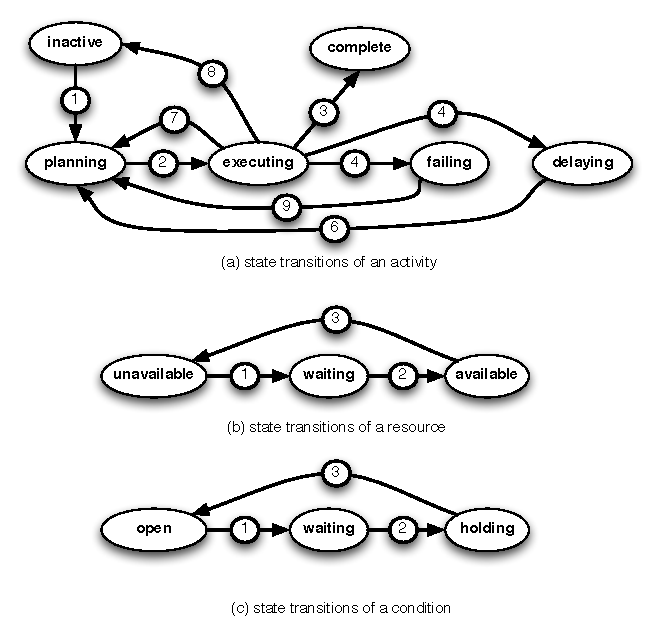
\includegraphics{state_transitions.pdf} 
	\caption{Types of node variables and possible values in a Bayesian network}
	\label{fig:state_transitions}
\end{figure}
% paragraph construction_of_bayesian_networks (end)
\paragraph*{Assignment of conditional probabilities} % (fold)
\label{par:assignment_of_conditional_probabilities}
Before any propagation commences, we need to assign the conditional probabilities for each node that form the conditional probability matrices. An element of the conditional probability matrix looks like $P(x_i|u_{1j_1}, ..., u_{nj_n})$, and gives the probability of state $i$ for node $x$ conditioned on the states of its parent nodes. For example, the conditional probability of an action node indicates the possibility of each state for this action, given the states of all the resources, conditions, actions that it depends on. 

In our study, we develop a set of heuristic rules to assign the initial conditional probabilities for each type of nodes, by evaluating the criticality of each parent node, and the opportunities for re-planning. For example, if a critical resource is needed for every possible way to perform an action, the state of the resource as \emph{failing} will definitely lead to the \emph{failing} of the action. However, if there are other possible plans to perform the action that do not require this resource, the probability of the action being failing will be decreased.

The assignment of conditional probabilities provides the system with the default reasoning capability to propagate state changes that can be later overwritten by human actors' interpretation. When a human actor changes the belief in the execution state of an action, the change will overwrite the system’s initial belief through the belief updating. Because of this interactive nature, the purpose of the initial probability assignment is just to provide a good guess about the propagation from the system's perspective and does not have to be perfectly accurate. 
% paragraph assignment_of_conditional_probabilities (end)

\paragraph*{Belief Updating} % (fold)
\label{par:belief_updating}
We follow Pearl’s belief propagation algorithm \cite{pearl1988probabilistic} to perform belief updating whenever a state change occurs. In this approach, the belief in each value of a node variable is divided into two parts: the part emerges from its ancestors and the part emerges from its descendants, and the final belief is ascribed by multiplying the two parts. As a result, the belief updating is performed as a bidirectional propagation process. 
\begin{enumerate}
	\item Starting at the node where the initial state change occurs, the system calculates how the state change will change the beliefs on each parent node. If the change on a parent node is significant, i.e. above a given threshold, the parent node becomes active, and will be further propagated to its parent. This is called \emph{causal} propagation since the updating is from a cause to an effect to indicate how a state change of the cause will lead to the change of the effect. 
	\item On the other hand, the belief updating can also calculated from an active node to their children. This is called \emph{evidential} propagation as the reasoning flows from evidence to hypothesis.
\end{enumerate}

In our approach, both the causal and evidential propagation will be performed. The causal propagation is used to provide the system's predicted state changes on the actions depending on the action associated with the initial state change. The evidential propagation occurs whenever a human actor modifies the system’s prediction on a given node and the system uses it as an evidence to trace back and revise the previous beliefs on other actions.
% paragraph belief_updating (end)

The result of the Bayesian network-based propagation will be used to enrich the event chain with anticipatory events. Starting from the node that the initial event is linked to, the system use the previous probability distribution before the propagation and the current values to perform the Cartesian product on each node. Each value in the new two-dimension table indicates the probability of each possible state change. If a significant state change has been detected (by comparing with pre-defined threshold), it will be added to the event chain as a new anticipatory event. For example, Figure \ref{fig:prob_state_change} shows the result of a propagation process on a parameter node. Before the propagation, the parameter had a high probability to be in the state of \emph{waiting}, and after the propagation, the probability distribution changed. By calculating the Cartesian product, we can find the most significant state change on the node is from \emph{waiting} to \emph{delay}, with a confidence level of $0.83808$. As a result, a new anticipatory event indicating that the state of this parameter has been changed from \emph{waiting} to \emph{delay} will be pushed into the event chain.
\begin{figure}[htbp] %  figure placement: here, top, bottom, or page
	\centering
	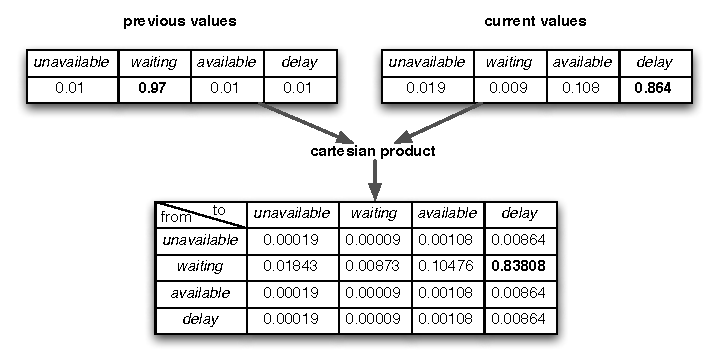
\includegraphics{prob_state_change.pdf} 
	\caption{An example of calculating state change probabilities}
	\label{fig:prob_state_change}
\end{figure}
% subsection propagation (end)
\subsection{An Example} % (fold)
\label{sub:an_example}
To demonstrate the knowledge updating process, we consider a simplified version of the victim rescue activity in the emergency response scenario to see how the PlanGraph model is updated through several consecutive events, and meanwhile the events are enriched into event chains. The task involved in this example is quite simple. Whenever a victim is found, it needs to be rescued by sending to a medical station for treatment. We assume there is only one station and one medical professional ($med$) working at it. There might be several drivers ($dr_1, dr_2, ...$) with rescue vehicles that can deliver the victim to the station.   

\paragraph*{Event 1: \emph{`NewVictim'}} % (fold)
\label{par:event_1_emph_newvictim}
The first event sent to the system is an external event reporting that a new victim has been found. The event has an event type \emph{`NewVictim'} and has several key attributes (e.g. id, occurrence time, location, required delivery time). Figure \ref{fig:update_example_event1} shows the knowledge updating process performed on this event.

\begin{enumerate}
	\item When the event is first sent to the system, the system attempts to associate it with any existing entities in the PlanGraph. Because this is the start of the activity, no association can be found. 
	\item Then the event is further processed in the assessment step, where the system checks whether the event can lead to changes on existing actions or trigger new action. By checking the association rules stored in the knowledge base, the system finds that every \emph{`NewVictim'} event will activate the goal to rescue the victim. Following this activation rule, the initial PlanGraph is generated with just one action node (\emph{`rescue'}) representing this new action to rescue the victim.
	\item After the assessment, the system finds that a new action has been added to the PlanGraph, which triggers the elaboration process. The system searches the knowledge base to find a recipe for the \emph{`rescue'} action, and extends the PlanGraph model with the parameters, conditions, and sub-actions. In this example, there is one parameter that is the \emph{`victim'} who needs to be rescued, one condition (\emph{`victimAtStation'}) that is the victim needs to be located at the medication station, and then the sub-action (\emph{`medicalTreat'}) to perform the medical treatment on the victim. As these subsidiary entities are also new to the PlanGraph, the elaboration continues on each of them. During the elaboration of the parameter, the system assigns it with the value from the input event. The condition is elaborated with a new action (\emph{`transport'}) to achieve it, which is further elaborated into subsidiary parameters and actions (\emph{`vehicle'}, \emph{`pickup'}, \emph{`deliver'}). During the elaboration of action \emph{`medicalTreat'} and action \emph{`transport'}, the system also looks for the potential actors who might be interested in these actions. Based on the actor $med$'s role as a medical professional, the system believes that $med$ has the potential intention ($pot.int$) and is able ($able$) to perform the \emph{`medicalTreat'} action. Similarly, the system believes all the drivers $dr_1, dr_2, ...$ have the potential intention ($pot.int$) and are able ($able$) to perform the \emph{`transport'} action.
	\item Because the event does not indicate any state change on current actions, the propagation is skipped.
\end{enumerate}

As we can see in Figure \ref{fig:update_example_event1}, after the knowledge updating process, the PlanGraph is updated to reflect the system's prediction on how the activity will be advanced. At the same time, the initial event is augmented with a new attribute pointing directly to the parameter node \emph{`victim'} in the PlanGraph.
\begin{figure}[htbp] %  figure placement: here, top, bottom, or page
	\centering
	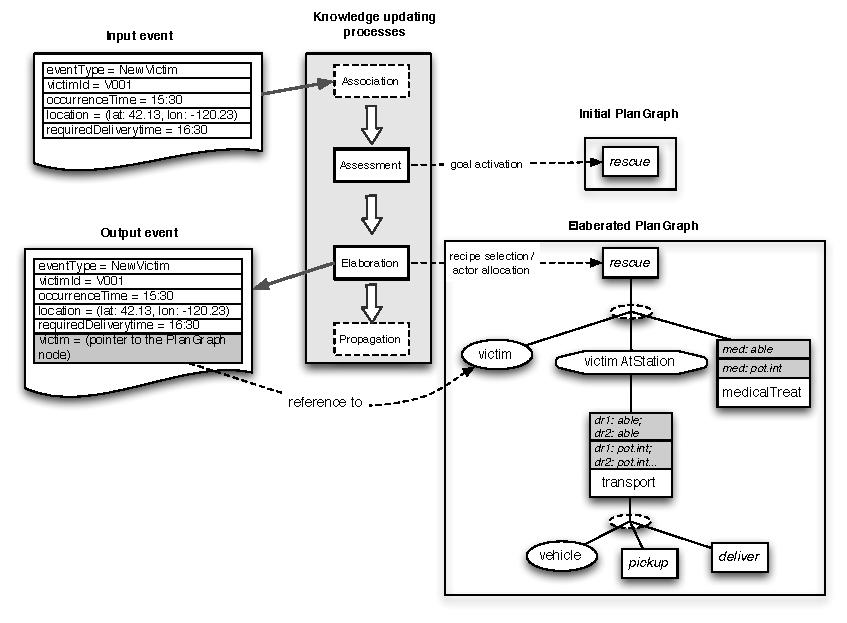
\includegraphics{update_example_event1.pdf} 
	\caption{The knowledge updating example (\emph{Event 1})}
	\label{fig:update_example_event1}
\end{figure}
% paragraph event_1_emph_newvictim (end)
\paragraph*{Event 2: \emph{`IntentionChange'}} % (fold)
\label{par:event_2_emph}
The second event is an internal event that is generated by the driver $dr_1$. After interpreting the first \emph{`NewVictim'} event, $dr_1$ intends to perform the \emph{`transport'} action to deliver this new victim to the medical station. As a result, he generates this \emph{`Intention'} event to update his intention on the \emph{`transport'} action from $pot.int$ to $int.to$. This \emph{`IntentionChange'} event has several key attributes, including the actor's id ($dr_1$), the action $dr_1$ intends to perform (\emph{`transport'}), and the intention type ($int.to$).

As the system receives this event, it first attempts to associate the event with any existing entities in the PlanGraph model. Because this is an intention event, the system traverses through the PlanGraph to search for any match between the action (\emph{`transport'}) mentioned in the event and the action nodes in the PlanGraph. As the system is able to find such a match, the system uses the information in the event to update $dr_1$'s intention level on action \emph{`transport'}. Meanwhile, the corresponding attributes of the actor and the action in the event are updated with reference to the corresponding nodes in the PlanGraph.

The knowledge updating process then proceeds to the following steps, but none of them leads to further changes in both the PlanGraph and the event itself. Figure \ref{fig:update_example_event2} shows the whole process performed on the second event.
\begin{figure}[htbp] %  figure placement: here, top, bottom, or page
	\centering
	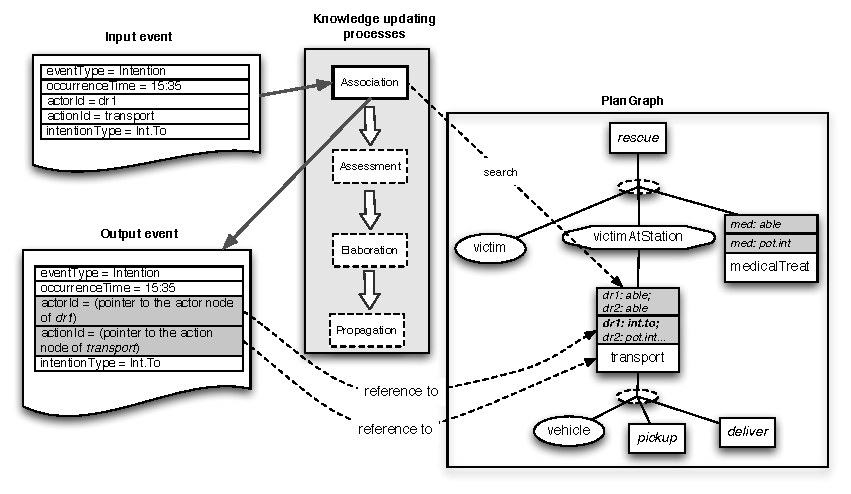
\includegraphics{update_example_event2.pdf} 
	\caption{The knowledge updating example (\emph{Event 2})}
	\label{fig:update_example_event2}
\end{figure}
% paragraph event_2_emph (end)

\paragraph*{Event 3: \emph{`FuelLevelLow'}} % (fold)
\label{par:event_3_}
The third event happens after $dr_1$ starts the action \emph{`transport'} and is on the way to pick up the victim. It is an external event indicating that the fuel level on driver $dr_1$'s vehicle is running extremely low. The event has an event type \emph{`FuelLevelLow'} and carries information about the driver, the vehicle, and the current fuel level. Figure \ref{fig:update_example_event3} shows the knowledge updating process performed on this event.

\begin{enumerate}
	\item When the event is first sent to the system, the system attempts to associate it with any existing entities in the PlanGraph model. Because this is an external event indicating an attribute change on an entity, the system traverses through the PlanGraph to search for any match between the entity (\emph{`vehicle'}) mentioned in the event and the nodes in the PlanGraph. When the system is able to find such a match, the system uses the information in the event to update the value attached to the parameter (\emph{`vehicle'}).
	\item Then the event is further processed in the assessment step, where the system checks whether the event can lead to changes towards the action performance. By checking the conditions attached with the parameter (\emph{`vehicle'}), the system finds that because of the low fuel level on the vehicle, the parameter becomes unavailable to perform the \emph{`transport'} action. As a result, a new state change event \emph{`ExecStateChange'} is derived to describe the execution state of the parameter, and is added to the output event chain.
	\item As no new action nodes are added to the PlanGraph, the elaboration process is skipped.
	\item Because a state change event has been derived in the assessment step, the system attempts to predict future state changes in the propagation step. A Bayesian network is constructed based on the current PlanGraph model and used to reason how likely the other entities in the PlanGraph will be impacted by the initial state change. After the Bayesian network-based reasoning, the system finds that $dr_1$'s action to pick up the victim (\emph{`pickup'}) is likely to change its state from \emph{executing} to \emph{delaying}, and a new anticipatory event describing this state change on the execution state of the \emph{`pickup'} action is generated, and added to the output event chain.
\end{enumerate}

As we can see in Figure \ref{fig:update_example_event3}, after the knowledge updating process, the initial event is augmented into an event chain with three events: the original external event \emph{`FuelLevelLow'}, the state change event on the parameter \emph{`vehicle'} derived in the assessment step, and the anticipatory event predicting the state change on the action \emph{`pickup'} in the propagation step. This example shows the idea that not only the knowledge representation of the collaborative activity, i.e. PlanGraph model is modified during the knowledge updating process, but also the original event is enriched with system generated knowledge.

\begin{figure}[htbp] %  figure placement: here, top, bottom, or page
	\centering
	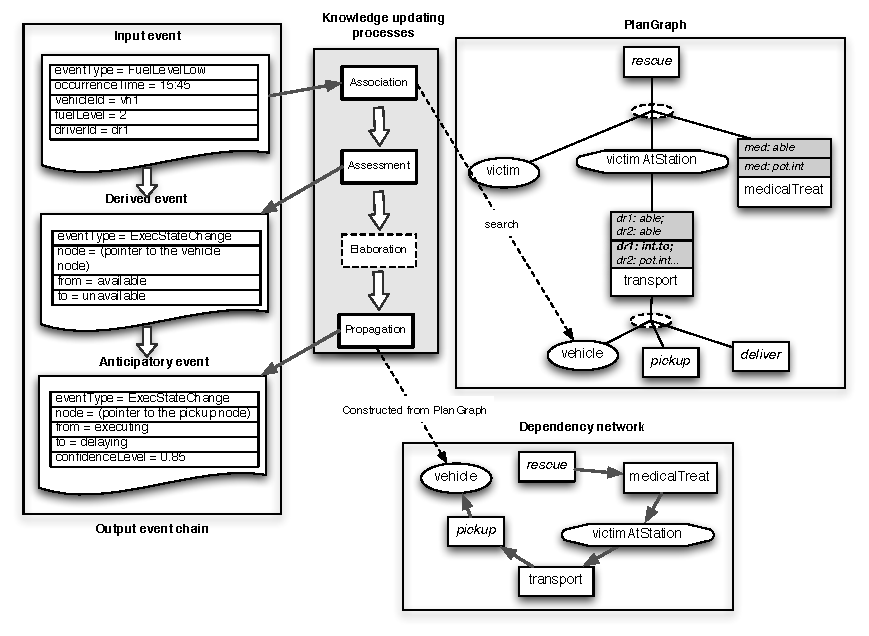
\includegraphics{update_example_event3.pdf} 
	\caption{The knowledge updating example (\emph{Event 3})}
	\label{fig:update_example_event3}
\end{figure}
% paragraph event_3_ (end)
% subsection an_example (end)
% section knowledge_updating_process (end)

\section{Discussion} % (fold)
\label{sec:knowledge_representation_discussion}
In this chapter, we first focus on the knowledge representation of collaborative activities. We employ the PlanGraph model to represent the entities and relations in collaborative activities, and then use this model to derive knowledge about local scopes of work and dependencies. The PlanGraph model exhibits some important characteristics that make it suitable to satisfy the three requirements for representing collaborative activities described in Section \ref{sub:computational_representation_of_the_field_of_work}.

\begin{enumerate}
   \item The PlanGraph model represents collaborative activities as hierarchically structured actions. The components of actions, parameters, conditions can be used to capture all the entities and the relations between them. With the knowledge represented in the PlanGraph, the local scopes and dependencies can also be easily identified. 
   \item A critical point made in the PlanGraph model is the emphasis on the development of collaborative activities. With the development of the activity, the PlanGraph model needs to be updated accordingly, so that it always  reflects the current state of the changing activities.
   \item Based on the formalization in SharedPlan theory, the PlanGraph model can be computationally implemented, and it provides a set of reasoning capabilities that can be operationalized to support computer reasoning.  
\end{enumerate}

Following that, we discuss the representation of events and identify the major event types supported in this study. The central idea of our approach is the interaction between these two knowledge components, which has been described in the knowledge updating process. On one hand, the various events are consumed by the computer system to update its PlanGraph-based representation of collaborative activities. On the other hand, the PlanGraph model enriches the events with more meaningful contextual information, which is used in next chapter to support event-driven awareness processes. 
% section knowledge_representation_discussion (end)
% chapter knowledge_reprsentation_and_updating (end)




 

